\chapter{Testing}
\label{chp:testing}
\noindent
This chapter describes the methods used for software testing.

\section{Feedbacks from surgeons}
\noindent
The development of this thesis has been conducted in close collaboration with cardiothoracic surgeons.
Through a series of iterative meetings and discussions, their insights have been fundamentals for ensuring the alignment with the requirements.
These collaborative sessions provided an opportunity to gather detailed feedback, which was then systematically integrated into the design and implementation phases.
This ongoing dialogue not only allowed for continuous improvement but also fostered a multidisciplinary approach.\\
Consequently, the iterative development process led to a solution that is both technologically robust and highly tailored to the specific needs and expectations of the end users.

\begin{figure}[ht]
  \centering
  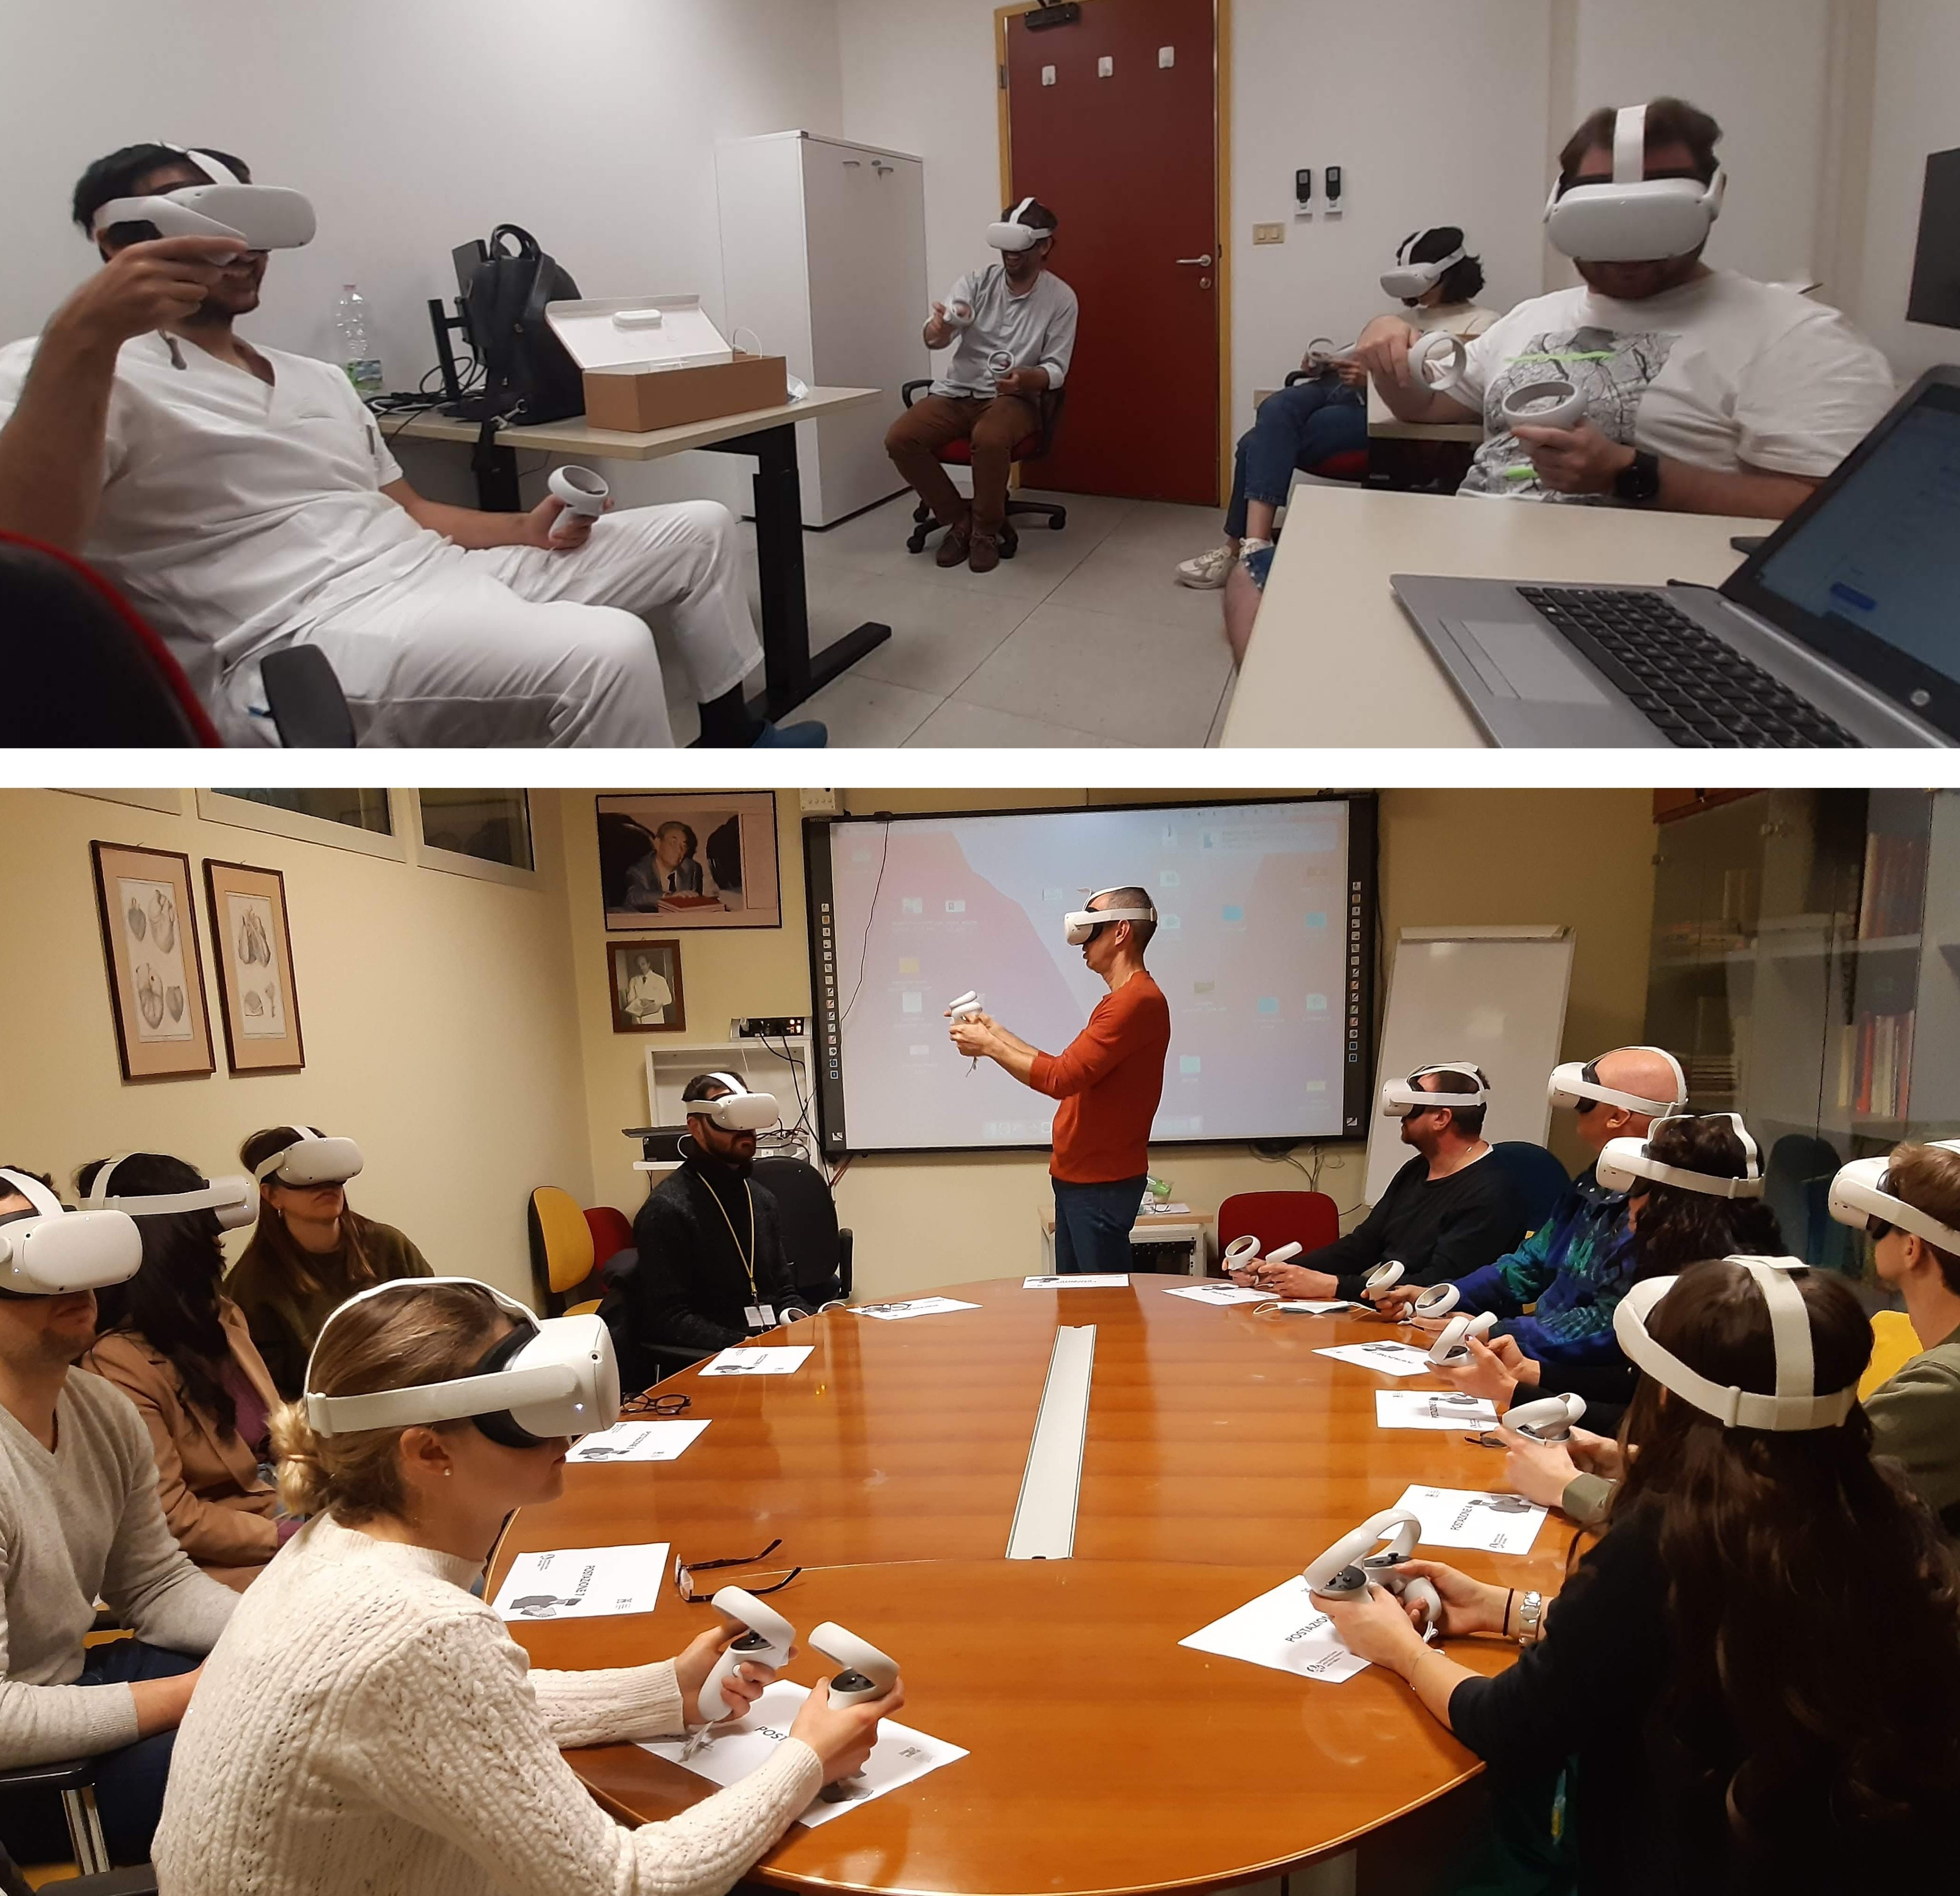
\includegraphics[width=0.96\textwidth]{testing.jpg}
  \caption{Testing session}
  \label{fig:testing}
\end{figure}

\section{Science4All}
\noindent
Science4All is a science outreach and inclusion software in Padua, aimed at making complex scientific topics accessible to a broad audience,
from young people to adults without a scientific background, with particular attention to people with disabilities or from disadvantaged backgrounds.\\
For the occasion, the \ac{VR} app was presented in the 3D printing section focused on medical applications. In a specially designed environment Fig.[\ref{fig:science4all}], we allowed children to try the \ac{HMD}, for many, it was their first time experiencing \ac{VR}. They had the opportunity to view a heart model, exploring both the exterior and interior in detail.
Both children and parents were captivated by the app capabilities and the medical use case for which it was developed.

\begin{figure}[ht]
  \centering
  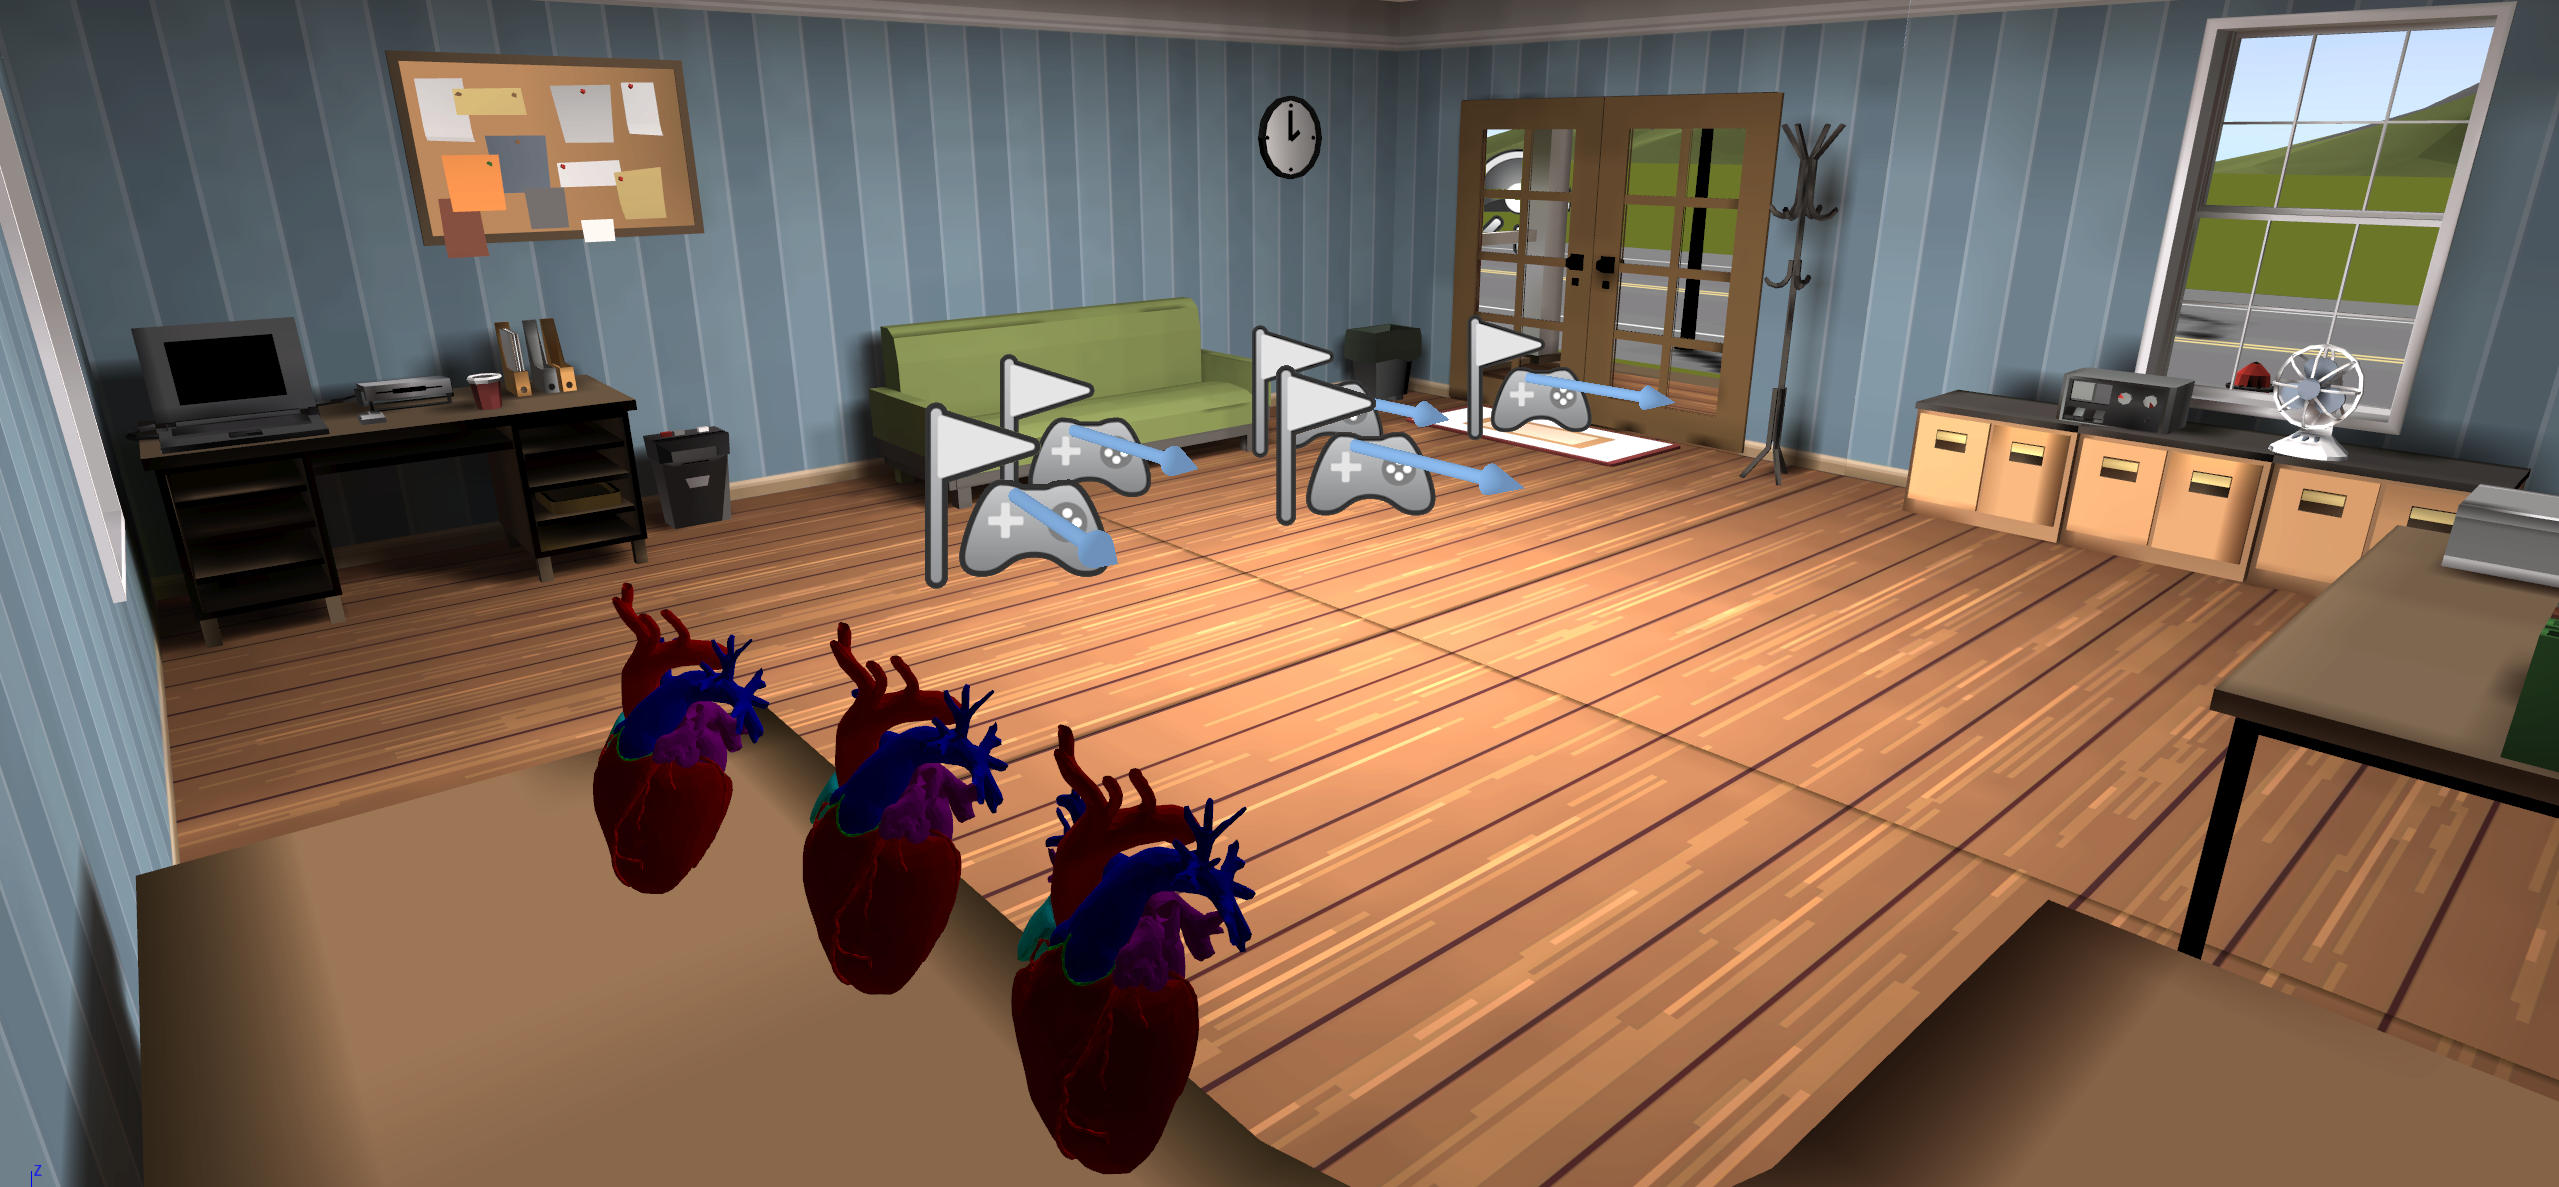
\includegraphics[width=0.96\textwidth]{vrScreenshot/science4all.png}
  \caption{Science4All environment}
  \label{fig:science4all}
\end{figure}